% Problem 6
\subsubsection{6.} 공정한 주사위를 5번 반복해서 던지는 게임을 한다.
\begin{itemize}
	\item[(1)] 5번 모두 짝수의 눈이 나올 확률을 구하라.
	\item[(2)] 5번 모두 서로 다른 눈이 나올 확률을 구하라.
\end{itemize}

\paragraph{Solution.}
\begin{itemize}
	\item[(1)] 공정한 주사위에서 짝수의 눈이 나올 확률은 $\dfrac{3}{6} = \dfrac{1}{2}$이므로, 5번 모두 짝수의 눈이 나올 확률은 $\left(\dfrac{1}{2}\right)^5=\dfrac{1}{32}$이다.
	\item[(2)] 2번째 시행에서 1번째와 다른 눈이 나올 확률은 $\dfrac{5}{6}$, 3번째 시행에서 1--2번째와 다른 눈이 나올 확률은 $\dfrac{4}{6}$, 4번째 시행에서 1--3번째와 다른 눈이 나올 확률은 $\dfrac{3}{6}$, 5번째 시행에서 1--4번째와 다른 눈이 나올 확률은 $\dfrac{2}{6}$이다. 따라서 구하고자 하는 확률은 $\dfrac{5}{6}\times\dfrac{4}{6}\times\dfrac{3}{6}\times\dfrac{2}{6}=\dfrac{5}{54}$이다.
\end{itemize}

% Problem 9
\subsubsection{9.} 주머니 안에 흰색 바둑돌이 4개, 검은색 바둑돌이 6개 들어있다. 꺼낸 바둑돌을 다시 주머니에 넣지 않는 방법으로 이 주머니에서 차례로 바둑돌 3개를 꺼낼 때, 다음을 구하라.
\begin{itemize}
	\item[(1)] 3개 모두 흰색일 확률
	\item[(2)] 차례로 흰색, 검은색, 그리고 흰색일 확률
\end{itemize}

\paragraph{Solution.}
\begin{itemize}
	\item[(1)] 1번째, 2번째, 3번째 시행에서 흰색 바둑돌을 고를 확률은 각각 $\dfrac{4}{10}$, $\dfrac{3}{9}$, $\dfrac{2}{8}$이다. 따라서 구하고자 하는 확률은 $\dfrac{4}{10}\times\dfrac{3}{9}\times\dfrac{2}{8}=\dfrac{1}{30}$이다.
	\item[(2)] 1번째, 2번째, 3번째 시행에서 차례로 흰색, 검은색, 그리고 흰색 바둑돌을 고를 확률은 각각 $\dfrac{4}{10}$, $\dfrac{6}{9}$, $\dfrac{3}{8}$이다. 따라서 구하고자 하는 확률은 $\dfrac{4}{10}\times\dfrac{6}{9}\times\dfrac{3}{8}=\dfrac{1}{10}$이다.
\end{itemize}

% Problem 11
\subsubsection{11.} 다음 회로의 각 스위치는 독립적으로 작동하며 1번 스위치가 ON이 될 확률은 $0.95$, 2번 스위치와 3번 스위치가 ON이 될 확률은 각각 $0.94$, $0.86$이라고 한다. 이 회로에 대하여 A와 B 두 지점에 전류가 흐를 확률을 구하여라.
\begin{center}
	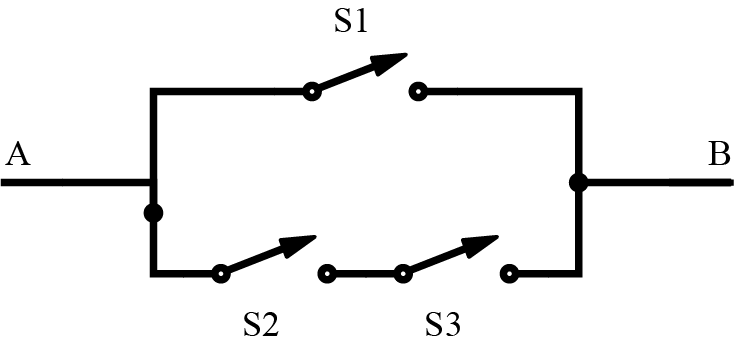
\includegraphics[width=0.5\columnwidth]{hw/1-3-diagram.png}
\end{center}

\paragraph{Solution.} 1번 스위치가 작동하거나, 2번과 3번 스위치가 동시에 작동하면 된다. 따라서 1번 스위치가 작동하는 사건을 $S_1$, 2번 스위치가 작동하는 사건을 $S_2$, 3번 스위치가 작동하는 사건을 $S_3$이라고 하면 구하고자 하는 확률은
\begin{align*}
	& P\left[S_1 \cup \left(S_2 \cap S_3\right)\right]\\
	=& P\left(S_1\right) + P\left(S_2 \cap S_3\right) - P\left[S_1 \cap \left(S_2 \cap S_3\right)\right]\\
	=& 0.95 + \left(0.94 \times 0.86\right) - \left(0.95 \times 0.94 \times 0.86\right)\\
	=& 0.99042
\end{align*}
이다.

% Problem 12
\subsubsection{12.} 위성 시스템은 두 개의 독립적인 백업용 컴퓨터(computer 2, computer 3)를 가진 컴퓨터(computer 1)에 의하여 조정된다. 정상적으로 computer 1은 시스템을 조정하지만 이 컴퓨터가 고장 나면 자동적으로 computer 2가 작동하고, computer 2가 고장 나면 computer 3이 작동한다. 그리고 세 컴퓨터가 모두 고장 나면 위성 시스템은 멈춘다고 한다. 그리고 각 컴퓨터들이 멈출 확률은 0.01이고, 이 컴퓨터들이 멈츄는 것은 역시 독립적이다. 이 때 각 컴퓨터들이 작동할 확률을 구하라. 그리고 위성 시스템이 멈출 확률을 구하라.

\paragraph{Solution.} 컴퓨터 1이 작동할 확률은 0.99이다.

컴퓨터 2가 작동할 확률은 컴퓨터 1이 작동하지 않으면서 컴퓨터 2가 정상적으로 작동할 확률이므로, $0.01 \times 0.99 = 0.0099$이다.

컴퓨터 3이 작동할 확률은 컴퓨터 1과 2가 작동하지 않으면서 컴퓨터 3이 정상적으로 작동할 확률이므로, $0.01 \times 0.01 \times 0.99 = 0.000099$이다.

위성 시스템이 멈출 확률은 컴퓨터가 모두 작동하지 않을 확률이므로, ${0.01}^3 = 0.000001$이다.

% Problem 17
\subsubsection{17.} AIDS 검사로 널리 사용되는 방법으로 ELISA 검사가 있다. 이 방법에 의하여 100,000명이 검사를 받았으며, 검사 결과 다음 표를 얻었다고 한다. 검사를 받은 사람들 중에서 임의로 한 명을 선정하였을 때, 다음을 구하라.

\begin{center}
	\begin{tabular}{c|r|r}
			 \hline
			 & AIDS 균 보균자 & AIDS 균 미보균자 \\
			 \hline
			 양성반응 & 4,535 & 5,255 \\
			 음성반응 & 125 & 90,085 \\
			 \hline
			 계 & 4,660 & 95,340 \\
			 \hline
	\end{tabular}
\end{center}

\begin{itemize}
	\item[(1)] 선정한 사람이 미보균자일 때, 이 사람이 양성반응을 보일 확률
	\item[(2)] 선정한 사람이 보균자일 때, 이 사람이 음성반응을 보일 확률
\end{itemize}

\paragraph{Solution.}
\begin{itemize}
	\item[(1)] $\dfrac{5255}{95340} \approx 0.05511$
	\item[(2)] $\dfrac{125}{4660} \approx 0.02682$
\end{itemize}

% Problem 19
\subsubsection{19.} 의학 보고서에 따르면 전체 국민의 7.5\%가 폐질환을 앓고 있으며, 그들 중 90\%가 흡연가라고 한다. 그리고 폐질환을 갖지 않은 사람 중에 25\%가 흡연가라 한다.
\begin{itemize}
	\item[(1)] 임의로 선정한 사람이 흡연가일 확률을 구하여라.
	\item[(2)] 임의로 선정한 흡연가가 폐질환을 가질 확률을 구하여라.
\end{itemize}

\paragraph{Solution.} 임의로 선정한 사람이 흡연가인 사건을 $A$, 폐질환을 앓고 있는 사건을 $B$라고 하자. 그러면 문제에서 $P\left(B\right) = 0.075$, $P\left(A\middle|B\right) = 0.90$, $P\left(A\middle|B^c\right) = 0.25$이다.

따라서 $P\left(A\middle|B\right) = \dfrac{P\left(A \cap B\right)}{P\left(B\right)} = 0.90$이므로 \[P\left(A \cap B\right) = 0.90P\left(B\right) = 0.0675\]

이고, 또한 $P\left(A\middle|B^c\right) = \dfrac{P\left(A \cap B^c\right)}{P\left(B^c\right)} = 0.25$이므로 \[P\left(A \cap B^c\right) = 0.25P\left(B^c\right) = 0.25\left(1 - 0.075\right) = 0.23125\]

임을 알 수 있다.

\begin{itemize}
	\item[(1)] 임의로 선정한 사람이 흡연가일 확률 $P\left(A\right) = P\left(A \cap B\right) + P\left(A \cap B^c\right) = 0.0675 + 0.23125 = 0.29875$
	\item[(2)] 임의로 선정한 흡연가가 폐질환을 가질 확률 $P\left(B\middle|A\right) = \dfrac{P\left(B\cap A\right)}{P\left(A\right)} =\dfrac{0.0675}{0.29875}\approx 0.22594$
\end{itemize}

% Problem 20
\subsubsection{20.} 세 공장 A, B, 그리고 C에서 각각 40\%, 30\%, 30\%의 비율로 제품을 생산한다. 그리고 이 세 공정라인에서 불량품이 제조될 가능성은 각각 2\%, 3\%, 5\%라 한다. 어떤 제품 하나를 임의로 선정했을 때, 다음을 구하라.

\begin{itemize}
	\item[(1)] 이 제품이 불량품일 확률
	\item[(2)] 임의로 선정된 제품이 불량품이었을 때, 이 제품이 A에서 만들어졌을 확률과 B에서 만들어졌을 확률
	\item[(3)] 임의로 선정된 제품이 불량품이었을 때, 이 제품이 A 또는 B에서 만들어졌을 확률
\end{itemize}

\paragraph{Solution.} 임의로 선정한 제품이 불량품인 사건을 $X$라고 하자. 그리고 임의로 선정한 제품이 각각의 공장에서 만들어졌을 사건을 $A$, $B$, $C$라고 하자.
\begin{itemize}
	\item[(1)] $P\left(A\right)P\left(X\middle|A\right) + P\left(B\right)P\left(X\middle|B\right) + P\left(C\right)P\left(X\middle|C\right) = 0.40\times0.02+0.30\times0.03+0.30\times0.05=0.032$
	\item[(2)] $P\left(A\middle|X\right) = \dfrac{P\left(A\cap X\right)}{P\left(X\right)} = \dfrac{0.40\times 0.02}{0.032} = 0.25$, $P\left(B\middle|X\right) = \dfrac{P\left(B\cap X\right)}{P\left(X\right)} = \dfrac{0.30\times 0.03}{0.032} = 0.28125$
	\item[(3)] 사건 $A$와 $B$는 독립이므로, $P\left(A\cup B\middle|X\right) = P\left(A\middle|X\right)+P\left(B\middle|X\right) = 0.53125$
\end{itemize}

% Problem 23
\subsubsection{23.} 두 기계 A와 B에 의하여 컴퓨터 칩이 생산되며, 기계 A의 불량률은 $0.08$이고 기계 B의 불량률은 $0.05$라고 한다. 두 기계로부터 각각 하나의 컴퓨터 칩을 선정하였을 때, 다음을 구하여라.

\begin{itemize}
	\item[(1)] 두 개 모두 불량품일 확률
	\item[(2)] 두 개 모두 양호품일 확률
	\item[(3)] 정확히 하나만 불량품일 확률
	\item[(4)] (3)의 경우에 대하여, 이 불량품이 기계 A에서 생산되었을 확률
\end{itemize}

\paragraph{Solution.} A에서 불량품을 선택한 사건을 $A$, B에서 불량품을 선택한 사건을 $B$라고 하자. 이 때 $P\left(A\right) = 0.08$, $P\left(B\right) = 0.05$이다. 또한 $A$와 $B$는 독립사건이다.

\begin{itemize}
	\item[(1)] $A$와 $B$는 독립이므로, $P\left(A\cap B\right) = P\left(A\right)P\left(B\right) = 0.004$
	\item[(2)] $P\left(A^c\cap B^c\right) = P\left(A^c\right)P\left(B^c\right) = 0.874$
	\item[(3)] 정확히 하나만 불량품일 확률은 (1)의 사건과 (2)의 사건의 여사건이다. 따라서 $1 - 0.004 - 0.874 = 0.122$
	\item[(4)] A에서 불량품이, B에서 양호품이 각각 생산될 확률은 $0.08\times 0.95=0.076$이다. 따라서 (3)이 일어났을 때 이런 상황이 발생할 확률은 $\dfrac{0.076}{0.122} \approx 0.623$이다.
\end{itemize}